\documentclass[11pt, a4paper, oneside]{report}

\pagestyle{plain}

\usepackage[utf8]{inputenc}
\usepackage[margin=0.8in]{geometry}
\usepackage{amsmath,amssymb,amsfonts,amsthm}
\usepackage{scrlayer-scrpage}
\usepackage{tikz}
\usepackage{graphics}
\usepackage[export]{adjustbox}
\usepackage{wrapfig}
\usepackage{hyperref}
\usepackage[
backend=biber,
style=alphabetic,
sorting=ynt
]{biblatex}
\addbibresource{refs.bib}

\usepackage{enumerate}
\pagestyle{scrheadings}
\usepackage{array}

\newcolumntype{L}[1]{>{\raggedright\let\newline\\\arraybackslash\hspace{0pt}}m{#1}}
\newcolumntype{C}[1]{>{\centering\let\newline\\\arraybackslash\hspace{0pt}}m{#1}}
\newcolumntype{R}[1]{>{\raggedleft\let\newline\\\arraybackslash\hspace{0pt}}m{#1}}

\begin{document}

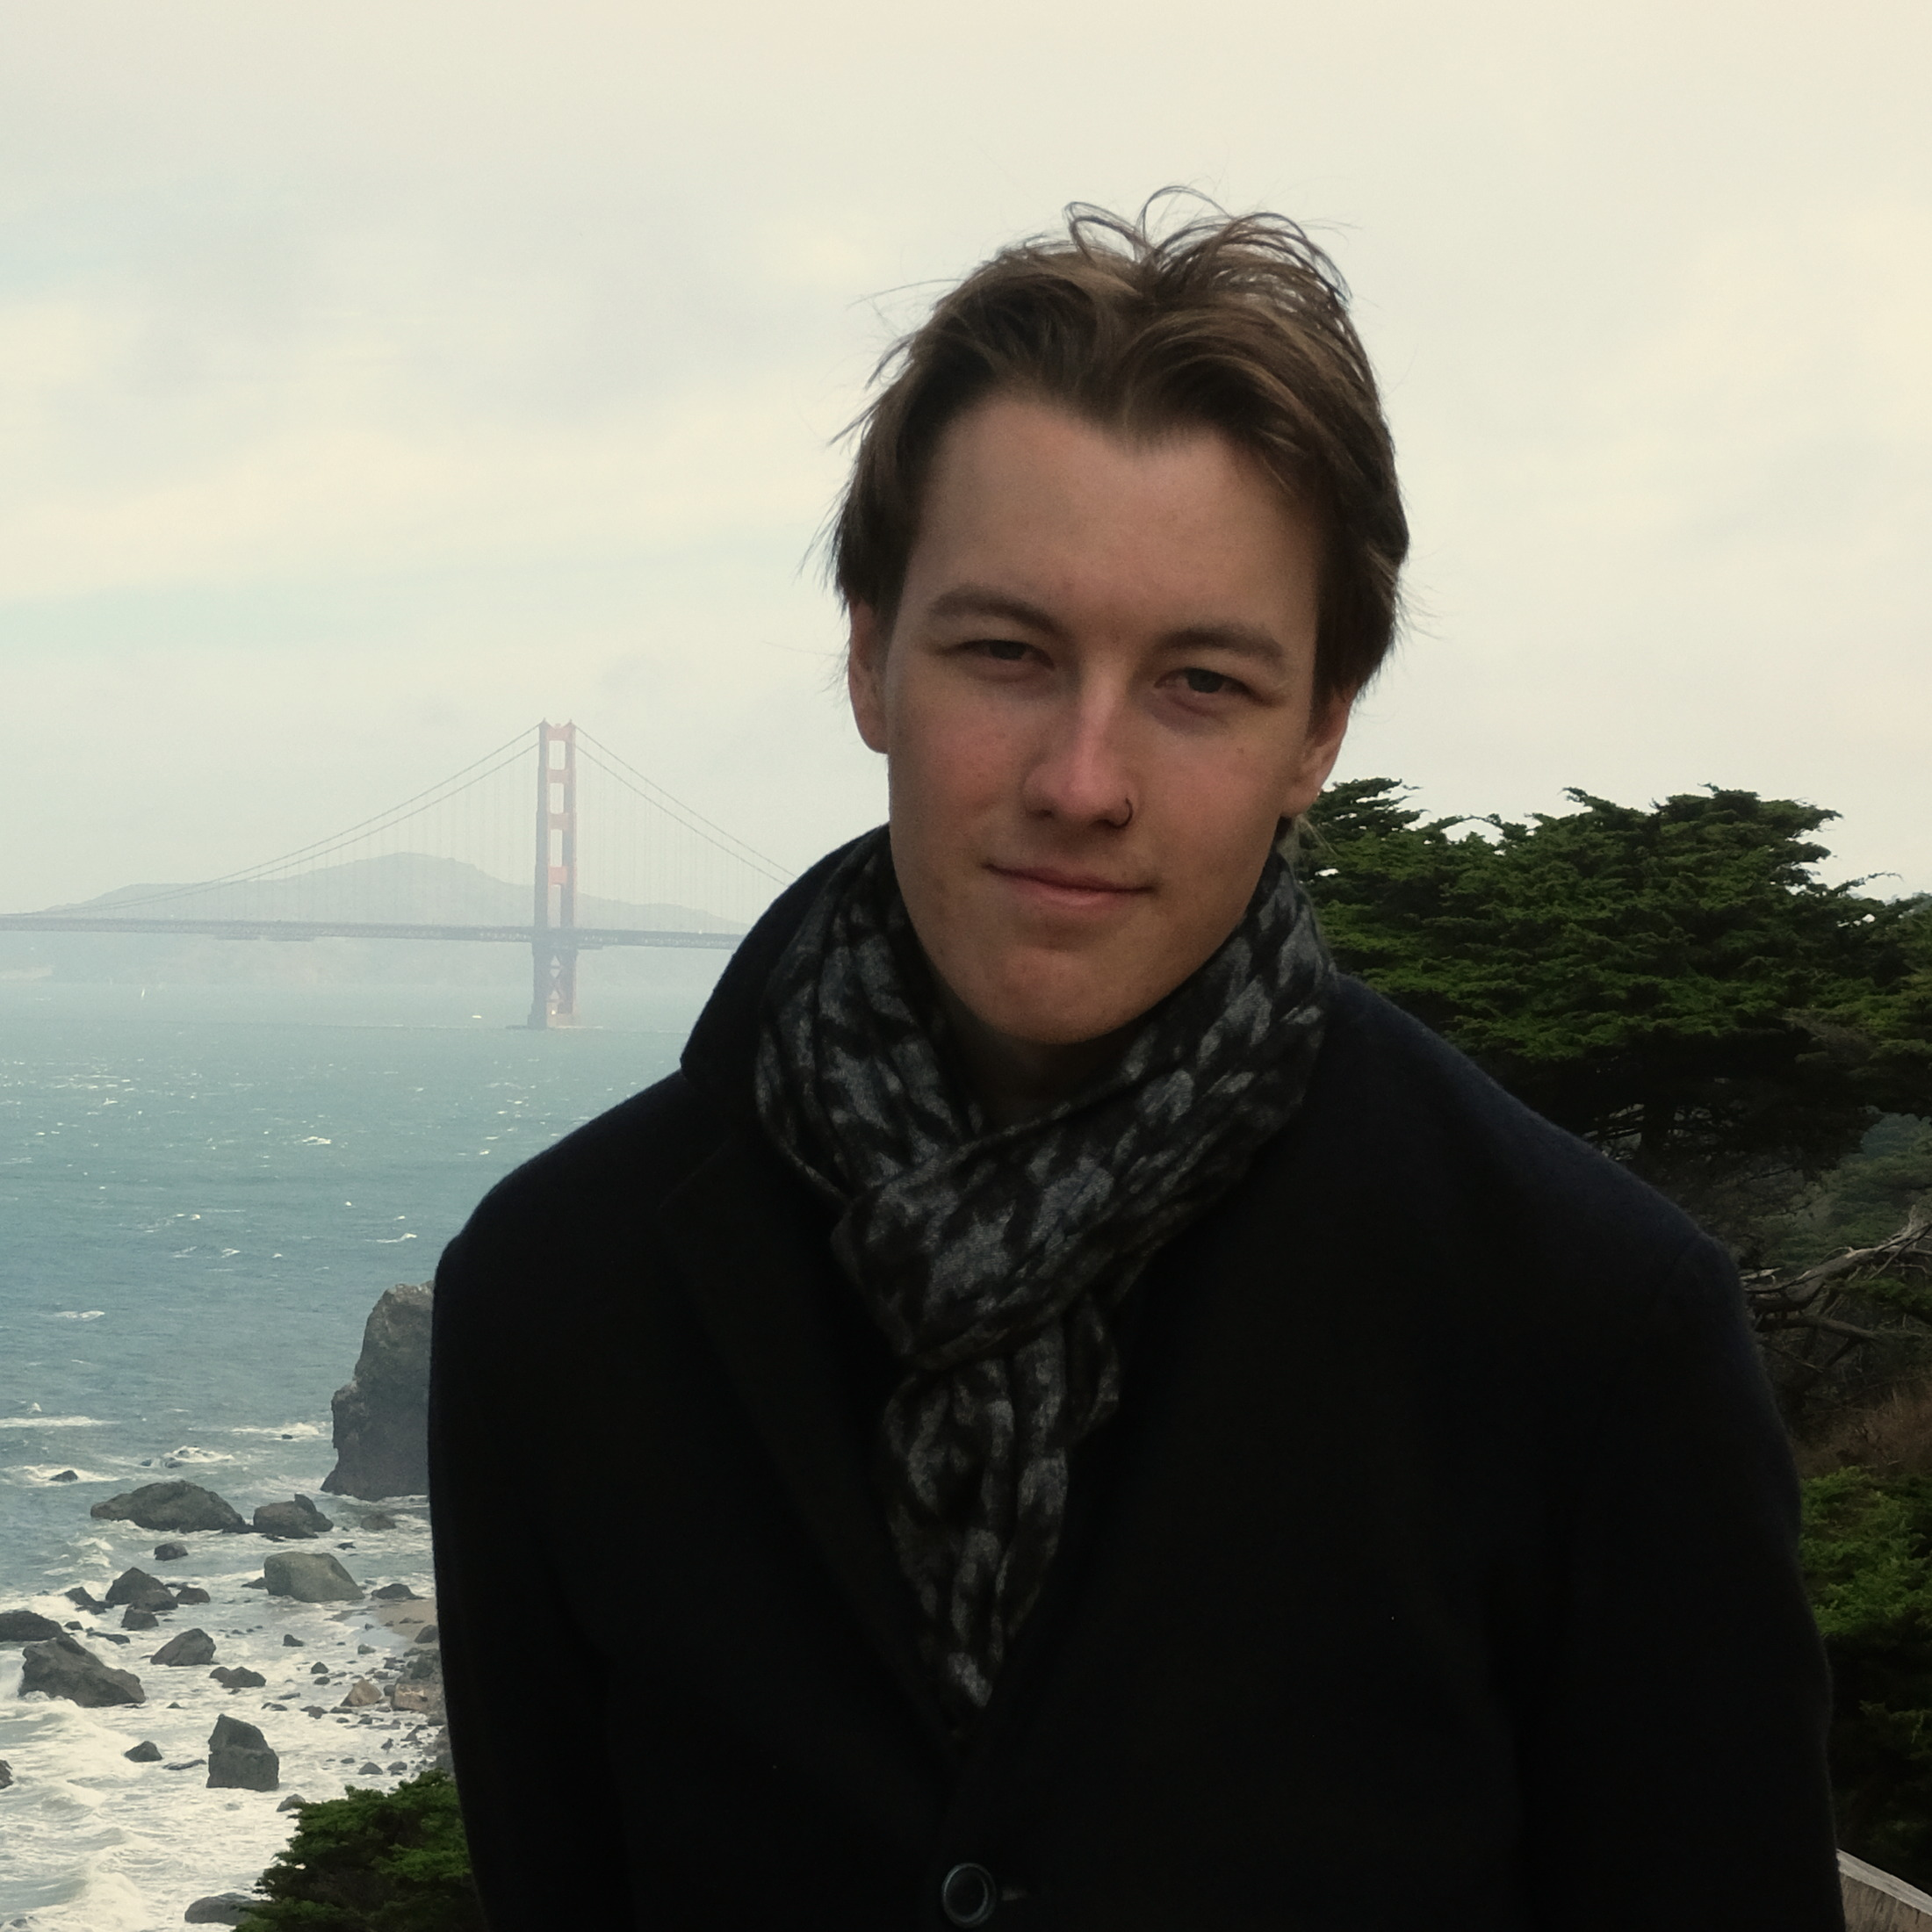
\includegraphics[width=0.3\linewidth, right]{Tassilo} 
\vspace*{-15em}
\begin{flushleft}
\hspace*{1.3em} \huge Tassilo Tanneberger
\vspace*{-0.5em}
\par\noindent\rule{0.6\textwidth}{0.4pt}
\end{flushleft}

\vspace*{-0.4em}

\begin{tabular}{l}
TUD Dresden University of Technology  \\
Faculty of Computer Science \\ 
Chair for Compiler Construction \\ 
\href{mailto: tassilo.tanneberger@tu-dresden.de}{\texttt{tassilo.tanneberger@tu-dresden.de}} \\
\href{https://tanneberger.me}{\texttt{https://tanneberger.me}} \\
\href{https://github.com/tanneberger}{\texttt{https://github.com/tanneberger}}
\end{tabular}

\par\noindent\rule{0.6\textwidth}{0.4pt}

\section*{Interests \& Research Focus}

Domain Specific Languages (DSLs), Distributed Systems, Embedded Systems, Scheduling Theory, RTOS, Deterministic Concurrency. 
Solving system architecture problems with languages.

\section*{Education}

\begin{tabular}{ R{3cm} L{10cm}}
	2021 - 2026 &  Study of Computer Science (Diploma) \\
							& TUD Dresden University of Technology \\ 
							&			\\
	5/2021			& Grammerschool with Grade 1.7
\end{tabular}


\section*{Professional Experience}

\begin{tabular}{R{3cm} L{12cm}}
	11/2021 	- now			& Research Student at the Chair for Compiler Construction, \\ 
										& TUD Dresden University of Technology \\ 
										& 																			\\
	4/2021 - 10/2021    & Engineer working on Tooling for Industrial Robots \\ 
										& Gesellschaft zur Förderung angewandter Informatik e.V. (GFaI)
\end{tabular}

\section*{Projects \&  Achievements}

\begin{tabular}{R{3cm} L{13cm}}

	2023 							& DD-IX Dresden Internet Exchange e.V. - Co-Founding and association that operates an Internet Exchange.  \href{https://dd-ix.net}{\texttt{https://dd-ix.net}} \\ & \\
		2022 							&  Transit Live Mapping Solutions - Reverse Engineering Radio Protocol used for controlling traffic lights in Germany and using this data to create live positional data of trams and buses. \href{https://tlm.solutions}{\texttt{https://map.tlm.solutions}} \\  & \\
		2021 							& Lingua-Franca - is a polyglot coordination language for reactive, concurrent, and time-sensitive applications. - Tasks ranged from optimizing the C++ runtime to develop a brand new package manager and built tool. \href{https://lf-lang.org}{\texttt{https://lf-lang.org}}
\end{tabular}

\section*{Publication List}

\nocite{*} 
\printbibliography[heading=none]

\end{document}
